\section{Filtriranje in glajenje}\label{sec:filtri}
%Filtri so zelo pomembni pri procesiranju signalov~\cite{smith1997scientist}. V našem delu jih uporabljamo za izločitev šuma izhodnih podatkov razvrščevalnika. 
Vhodne podatke obdelujemo bodisi z izračunom optičnega toka, bodisi s izračunom prostorskega toka za vsako sliko zaporedja slik, oziroma par slik. Ocena energijske porabe ni nikakor omejena med posameznimi slikami, zato vsebuje veliko šuma. Smiselno je, da zagotovimo časovno kontinuiteto ali s filtriranjem ali z glajenjem rezultatov porabe energije.

Izbrani filtri izhajajo iz družine filtrov tekočega povprečja, saj so ti najbolj optimalni za zmanjševanje šuma~\cite{smith1997scientist}. Splošna enačba filtra tekočega povprečja je~\eqref{eq:filter-tekocega-povprecja}, kjer je $x(i)$ i-ti vzorec vhodnega signala, $y(i)$ i-ti vzorec izhodnega signala in $M$ število vzorcev, ki jih uporabimo za filtriranje ali drugače, širina jedra filtra~\cite{smith1997scientist}.

\begin{equation}
y(i) = \frac{1}{M} \sum_{j=0}^{M-1} x(i + j)
\label{eq:filter-tekocega-povprecja}
\end{equation}

Prvi filter, ki je bil testiran, je Kalmanov filter. Zaradi slabih rezultatov in težav pri modeliranju hitrih sprememb porabe energije, ki so v številnih športih norma, smo prešli na Gaussov filter (glajenje), kar je dalo zadovoljive rezultate. Ker pridobivamo rezultate v absolutnem realnem času, zamuda, ki jo povzroča Gaussovo glajenje, ni kritična. Oba filtra sta podrobneje opisana v nadaljevanju.

%digitalni filtri so zelo pomemnbi pri digitalnem procesiranju signalov. filtre uporabljamo za dve stvari: signal separation and signam restoration. Prva se uporablja ko imamo signal ki je kontaminiran z interferenco, šumom ali drugimi signali. 

%signal restoration se uporablja ko je bil signal distorted in some way recimo debluring of an image.

%vsak filter im a impulze resonse step response in frekvenčni odziv. filter implementiramo tako da uporabmo konvolucijo z vhodnim signalom. 

%moving average filters
%optimalen za reducing random noise while retaining a sharp step response. najboljši za signale v časovnem prostoru.  -> gaussov filter -> frekvenčni odziv ravno tako gaussian  

\subsection{Digitalni Kalmanov filter}\label{sec:kalmanov-filter}
Kalmanov filter je sestavljen iz modela gibanja, merilnega modela in algoritma, s katerim izračunamo novo stanje modela gibanja~\cite{trucco1998introductory}.

\subsubsection{Model gibanja}
Gibanje modeliramo z vektorjem stanj $\vec{x}(k)$ na koraku $k$~\cite{trucco1998introductory}. Vektor stanj je predstavljen v enačbi~\eqref{eq:vektor-stanj}. Za stanja si običajno izberemo tiste spremenljivke gibanja $s_i(k)~\forall i = 1,2,\ldots \land k = 0, 1,\ldots$, ki jih opazujemo (npr. pozicija, hitrost, pospešek).

\begin{equation}
\vec{x}(k) = \begin{bmatrix}
					s_1(k) & s_2(k) & \ldots
\end{bmatrix}^\top
\label{eq:vektor-stanj} 
\end{equation}


Model gibanja je vektorska enačba~\eqref{eq:model-gibanja}, ki govori o razvoju modela gibanja skozi diskretni čas $k = 0,1,\ldots$~\cite{trucco1998introductory}. Diskretni čas oziroma koraki morajo biti dovolj majhni, da zajamemo dinamiko sistema. $\vec{A}$ je matrika prehajanja stanj in $\vec{G}$ matrika vhodnih parametrov $\tilde{s}_i~\forall i = 1,2,\ldots$ v vektorju $\vec{u}(k)$~\eqref{eq:vhodni-parametri}. 



\begin{equation}
\vec{x}(k) = \vec{A} \vec{x}(k-1) + \vec{G} \vec{u}(k)
\label{eq:model-gibanja}
\end{equation}

\begin{equation}
\vec{u}(k) = \begin{bmatrix}
					\tilde{s}_i(k) & \tilde{s}_i(k) & \ldots
			\end{bmatrix}^\top 
\label{eq:vhodni-parametri}
\end{equation}

$\vec{w}(k-1)$ predstavlja Gaussov šum $\mathcal{N}$ modela gibanja s srednjo vrednostjo $0$ in kovariančno matriko $\vec{Q}$, kot je prikazano v enačbi~\eqref{eq:sum-modela-gibanja}~\cite{trucco1998introductory}.

\begin{equation}
 \vec{w}(k) \sim \mathcal{N}\left(0,\vec{Q}\right)
 \label{eq:sum-modela-gibanja}
\end{equation}

Modeliranje šuma je ekvivalentno določevanju uteži upoštevanja modela v Kalmanovem algoritmu. Večji je šum, večja je negotovost modela, zato bo njegov vpliv na določitev novega stanja manjši~\cite{trucco1998introductory}.


\subsubsection{Merilni model}
Pri Kalmanovemu filtriranju predvidevamo, da ob vsakem časovnem trenutku dobimo meritev stanja $\vec{z}(k)$, ki je, realno gledano, pošumljena z Gaussovim šumom~\cite{trucco1998introductory}. Merilni model lahko predstavimo z vektorsko enačbo~\eqref{eq:merilni-model}, kjer je $\vec{H}$ merilna matrika in $\vec{\nu}(k)$ vektor Gaussovega šuma $\mathcal{N}$ s srednjo vrednostjo $0$ ter kovariančno matriko $\vec{R}$~\eqref{eq:sum-merilnega-modela}.


\begin{equation}
 \vec{z}(k) = \vec{H} \vec{x}(k) + \vec{\nu}(k)
 \label{eq:merilni-model}
\end{equation}

\begin{equation}
\vec{\nu}(k) \sim \mathcal{N} \left( 0, \vec{R} \right)
\label{eq:sum-merilnega-modela}
\end{equation}


Kot pri modelu gibanja tudi tu z modeliranjem šuma vnašamo določeno stopnjo negotovosti, ki vpliva na upoštevanje modela pri izračunu novega stanja~\cite{trucco1998introductory}.


\subsubsection{Algoritem}
S Kalmanovim algoritmom želimo čimbolj natančno določiti naslednjo oceno stanja sistema $\hat{\vec{x}}(k+1)$, pri čemer uporabimo trenutno meritev $\vec{z}(k)$ in trenutno oceno stanja $\hat{\vec{x}}(k)$~\cite{trucco1998introductory}. 

Jedro algoritma Kalmanovega filtra temelji na izračunavanju kovariančne matrike stanja $\vec{P}$ in matrike ojačanja filtra $\vec{K}$~\cite{trucco1998introductory}. Kovariančna matrika stanja predstavlja oceno vnosa napake zaradi šumnih modelov. Predstavlja šum celotnega sistema. Z ojačanjem določimo, kaj bolj vpliva na novo oceno stanja. To je bodisi trenutna ocena stanja bodisi trenutna meritev.

Algoritem lahko razdelimo na tri področja, in sicer: predikcijo, inovacijo in korekcijo~\cite{trucco1998introductory}.

\paragraph{Predikcija}
V predikciji določimo trenutno oceno stanja $\hat{\vec{x}}^-(k)$ po enačbi~\eqref{eq:ocena-stanja} in a priori kovariančno matriko stanja $\vec{P}^-(k)$ po enačbi~\eqref{eq:apriori-p}.

\begin{equation}
	\hat{\vec{x}}^-(k) = \vec{A} \hat{\vec{x}}(k-1) + \vec{G} \vec{u}(k)
    \label{eq:ocena-stanja}
\end{equation}

\begin{equation}
	\vec{P}^-(k) = \vec{A} \vec{P}(k-1) \vec{A}^\top + \vec{Q}
    \label{eq:apriori-p}
\end{equation}

\paragraph{Inovacija}
V koraku inovacije izberemo trenutno meritev $\vec{z}(k)$ iz nabora meritev. Merilno napako $\vec{e}$ določimo po enačbi~\eqref{eq:napaka}, kjer drugi člen predstavlja oceno meritve. Kovarianco inovacije $\vec{S}$ izračunamo po~\eqref{eq:kovarianca-inovacije}. Gre za pomožno matriko, ki jo uporabljamo za izračun ojačanja v naslednjem koraku.

\begin{equation}
	\vec{e}(k) = \vec{z}(k) - \vec{H} \hat{\vec{x}}^-(k)
    \label{eq:napaka}
\end{equation}

\begin{equation}
\vec{S}(k) = \vec{H} \vec{P}^-(k) \vec{H}^\top + \vec{R}
\label{eq:kovarianca-inovacije}
\end{equation}

\paragraph{Korekcija}
V zadnjem koraku najprej izračunamo ojačanje filtra $\vec{K}$ po enačbi~\eqref{eq:ojacanje}. Sledi določitev a posteriori ocene stanja $\hat{\vec{x}}(k)$ po~\eqref{eq:aposteriori-stanje} in a posteriori kovariančne matrike stanje $\vec{P}(k)$ po~\eqref{eq:aposteriori-p}, kjer je $\vec{I}$ identiteta.

\begin{equation}
\vec{K}(k) = {\vec{P}^-(k) \vec{H}^\top} ~/~ {\vec{S}(k)}
\label{eq:ojacanje}
\end{equation}

\begin{equation}
\hat{\vec{x}}(k) = \hat{\vec{x}}^-(k) + \vec{K}(k) \vec{e}(k)
\label{eq:aposteriori-stanje}
\end{equation}

\begin{equation}
\vec{P}(k) = \left( \vec{I} - \vec{K} \vec{H} \right) \vec{P}^-(k)
\label{eq:aposteriori-p}
\end{equation}








\subsection{Gaussov filter}\label{sec:gaussov-filter}
Gaussov filter $g$ je opredeljen z enačbo~\eqref{eq:gauss}, kjer je $x$ vzorec in $\sigma$ standardni odklon. 


\begin{equation}
g(x) = \frac{1}{\sqrt{2 \pi} \sigma} \mathrm{e}^{-\frac{x^2}{2 \sigma^2}} 
\label{eq:gauss}
\end{equation}


Primer filtra s standardnim odklonim $\sigma = 5$ je prikazan na sliki~\ref{fig:gauss}.

\begin{figure}[!htb]
\centering
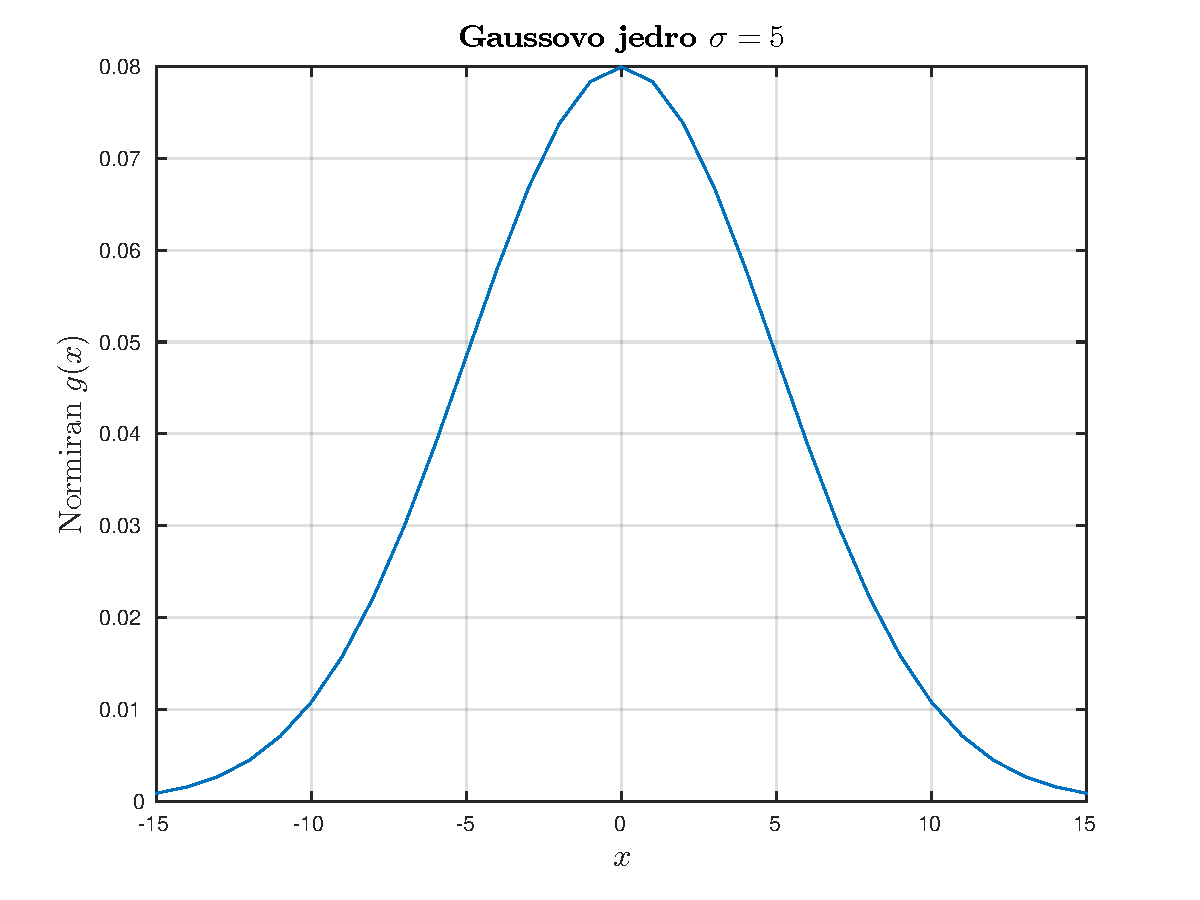
\includegraphics[width=0.7\columnwidth]{gauss-kernel-sl}
\caption[Gaussovo jedro s standardnim odklonom $\sigma=5$]{Gaussovo jedro s standardnim odklonom $\sigma=5$. }
\label{fig:gauss}
\end{figure}


Gaussov filter je vrsta filtra tekočega povprečja, ki je zelo primeren za izločevanje odvečnega šuma~\cite{smith1997scientist}. Ker je karakteriziran z impulznim odzivom, ki je simetričen okoli ničelnega vzorca, gre za vrsto filtra z ničelno fazo. To pomeni, da je faza v frekvenčnem prostoru vedno $0$~\cite{smith1997scientist}. Ker imamo pri takih filtrih negativne indekse, ga težje uporabljamo. 

Običajno filtre uporabljamo v rekurzivni obliki, saj je računanje hitrejše. Impulzni odziv rekurzivnega filtra ni simetričen, zato ima nelinearno fazo~\cite{smith1997scientist}. To pomanjkljivost lahko odpravimo z uporabo dvosmernega filtriranja.

Pri \emph{dvosmernem filtriranju} najprej filtriramo iz leve proti desni in nato iz desne proti levi~\cite{smith1997scientist}. Dobljena signala združimo in dobimo pravilen rezultat.


